\chapter{Systembeskrivelse}
Med udgangspunkt i projektformuleringen kommer dette projekts endelige system til at bestå af en software- og hardwaredel, der kan tilsluttes et måleobjekt, hvorpå et blodtryk kan måles. Systemet skal kunne implementeres i forskningsmiljøer, hvor en eller flere forskere ønsker at analysere målte blodtrykssignaler. Visionen er, at systemet skal være let tilgængeligt og effektivt, hvilket vil komme til udtryk ved, at systemet fungerer stabilt.

I dette projekt realiseres en prototype af systemet. Flere dele af systemet udvikles ud fra forsimplede metoder ift. hvordan det vil være optimalt at implementere dem i virkeligheden. Her tænkes på hardware- såvel som softwareelementer. Hardwaren i prototypen realiseres på et Veroboard, så det er muligt at tage den med sig, samt er mere holdbar over tid. Softwaren i prototypen består af flere moduler. Disse er opbygget efter principperne i en trelagsmodel. Dette er valgt for, at skabe et overblik over hvilke dele af software-koden, der har ansvaret for de enkelte funktionaliteter i systemet.

Hardwaren består af en forstærker og et filter. Forstærkerens opgave består i at forstærke det analoge signal fra maksimalt 11 mV til 5 V. Filteret sørger for at filtrere unødigt støj fra det analog signal. Signalændringen fra måleobjektet til visning af signal på en graf er skitseret herunder. Det skal pointeres at dette kun er en skitse for at skabe overblik, derfor er flere processer i softwaren udeladt af diagrammet. 
\begin{figure}[H]
	\centering
	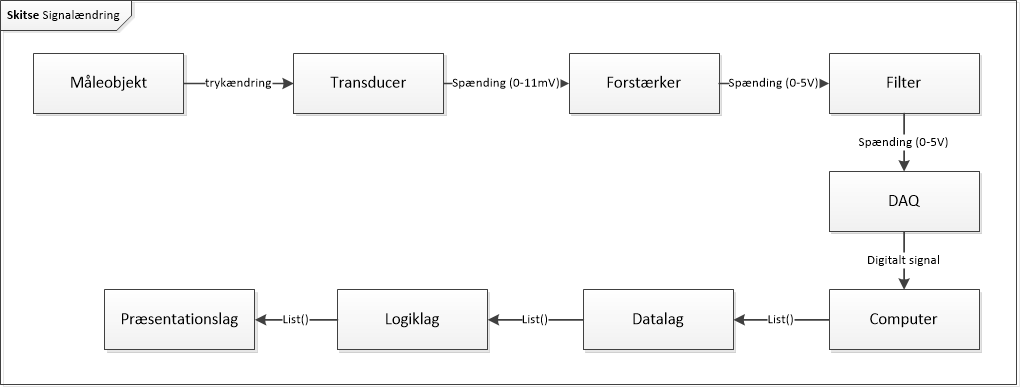
\includegraphics[width=1.0\textwidth]{Figurer/Signalandring}
	\caption{Skitse af signalændring}
	\label{fig:signalaendring}
\end{figure}
Database-laget består af en lokal database, samt indhentningen af blodtrykssignalet fra hardwaren. I den lokale database gemmes det indhentede blodtrykssignal i en tabel. Signalet gemmes med et tidsstempel, samt under et filnavn sammensat af et autogenereret Id og Forsøgsnavn, som forskeren indtaster på brugergrænsefladen ved begyndelsen af en måling. \\
Logik-laget er handlingslaget, og alt kommunikation til de resterende lag går gennem dette lag. Laget indeholder flere klasser, der indeholder metoder til indhentning af systoliske, diastoliske og puls værdier, ud fra det indhentede blodtrykssignal. Derudover indeholder laget også klasser, der har ansvaret for at foretage en filtrering af signalet når dette er valgt. \\ 
Præsentations-laget er forskerens vej ind i systemet, dette lag har til ansvar, at udskrive valgt data på brugergrænsefladen og at registrere tryk på knapper. 

Systemet skal udadtil have en brugergrænseflade i form af en touch skærm eller almindelig computerskærm med tilhørende tastatur. Det er denne skærm som den primære aktører, forskeren, interagerer med. Det tilstræbes, at opbygge brugergrænsefladen simpelt og efter forskerens logik, så opbygningen giver mening for systemets bruger. Efter indhentning af blodtrykssignal er systemet i stand til grafisk at vise signalet kontinuerligt, samt udskrive blodtrykssignalets systoliske, diastoliske og puls værdier. 
